\documentclass[]{article}

%opening
\title{Detecting Structure in Graphical Data}
\author{Lawrence Tray \\ Ioannis Kontoyiannis}

%packages
\usepackage[margin=0.5in]{geometry}
\usepackage{graphicx}
\usepackage{amsmath}
\usepackage{amssymb}
\usepackage{hyperref}
\usepackage{caption}
\usepackage{subcaption}
\usepackage{mathtools}
\usepackage{parskip}
\usepackage{fancyvrb}
\usepackage{bbm}

%bibliography
\usepackage[backend=bibtex]{biblatex}
\addbibresource{interim-sources.bib}

%package setup
\graphicspath{{./img/}}
\DeclareMathOperator*{\argmax}{arg\,max}
\DeclareMathOperator*{\argmin}{arg\,min}

%custom commands
\newcommand{\dft}{\mathcal{F}}
\newcommand{\idft}{\mathcal{F}^{-1}}
\newcommand{\Xcal}{\mathcal{X}}
\newcommand{\Dcal}{\mathcal{D}}
\newcommand{\cmplx}{\mathbb{C}}
\newcommand{\E}{\mathbb{E}}
\newcommand{\Gaussian}{\mathcal{N}}
\newcommand{\Gcal}{\mathcal{G}}
\newcommand{\Vcal}{\mathcal{V}}
\newcommand{\Ecal}{\mathcal{E}}
\newcommand{\pbold}{\boldsymbol{p}}
\newcommand{\sigmabold}{\boldsymbol{\sigma}}
\newcommand{\lik}{\mathcal{L}}
\newcommand{\kl}{\mathcal{D}}
\newcommand{\Integers}{\mathbb{Z}}
\newcommand{\SBM}{\textrm{SBM}}
\newcommand{\iid}{\stackrel{iid}{\sim}}
\newcommand{\one}{\mathbbm{1}}
\newcommand{\figwidth}{0.55\linewidth}


% definition
\newtheorem{definition}{Definition}[section]
\newtheorem{theorem}{Theorem}[section]
\newtheorem{corollary}{Corollary}[theorem]
\newtheorem{lemma}[theorem]{Lemma}


\begin{document}

\maketitle

\begin{abstract}
So the agenda for today. I will take you through my exploratory work around the field in rough chronological order. We’ll start off with the fundamentals of hypothesis testing. I will then introduce you to the most commonly used graphical model and talk about the ways of verifying structure in a graph with labelled nodes. However, that is not sufficient as we may want to detect structure in an unlabelled graph. Finally I’ll talk about the future direction of the project.
\end{abstract}

\tableofcontents

\section{Introduction}

There is a wealth of graphical data in the world and more is being produced each second; social networks, website hyperlinks and academic collaborations are just some examples of this data. There is a wealth of algorithms developed to analyse graphical data. Nevertheless, that same principled framework we have for querying classical data (hypothesis testing) is less developed for graphical data. Do my friends vote the same way I do or do researchers collaborate with those of the same gender? We want to answer these questions and not only that, we wish to report our confidence in the answers. To that end there is space to expand the hypothesis testing framework to graphs.

\section{The Stochastic Block Model}

The most popular graphical model in industry and indeed academia is called the Stochastic Block Model (SBM). We use a definition adapted from Abbe \cite{Abbe}.

\begin{definition}
	\label{defn:sbm}
	Let $n \in \Integers^+$ be the number of vertices and $k \in \Integers^+$ be the number of communities in an SBM graph. We define a probability vector $\pi = [\pi_1, \pi_2 \dots \pi_k]^T$ to be the prior on the k-communities. Each vertex $v \in \Vcal = \{1, 2 \dots N\}$ has a community label $X_v \in \{1, 2 \dots n\}$. Let $W$ be a symmetric $k \times k$ matrix with entries in $[0,1]$ called the connectivity matrix. We say that the pair $(X, \Gcal) \sim \textrm{SBM}(n, \pi, W)$ if X is an $N$-dimensional vector with each component independently distributed as the community prior $X_v \sim \pi$ and $\Gcal$ is an $N$-vertex graph where each pair of vertices $(i, j)$ is connected with probability $p(i \leftrightarrow j) = W_{X_i, X_j}$ independently of other pairs of vertices. Lastly, we define the community sets as $\Omega_i = \Omega_i(X) \coloneqq \{v \in \Vcal : X_v = i\}$ which contains all vertices belonging to community $i$.
\end{definition}

Though the definition of the SBM is simple, it allows for very deep and rich analysis of graphical datasets. For certain problems it helps to define the symmetric SBM.

\begin{definition}
	\label{defn:sym-sbm}
	The symmetric SBM is a special case denoted by $\textrm{SSBM}(n, k, q_{in}, q_{out}) \equiv \textrm{SBM}(n, p, W)$ if the community prior $p$ is uniform ($p_i = 1/k$ for $i \in \{1, 2, \dots k\}$) and $W_{ij}$ takes only two values, one on diagonal and another off diagonal such that $W_{ij} = q_{in}$ for $i=j$ and $W_{ij} = q_{out}$ for $i \neq j$.
\end{definition}

\section{Verifying Structure}

Armed with this definition we tackle the simplest problem in structure verification. Given an undirected graph $\Gcal$ and vertex-labels $X$, we wish to determine whether the two communities $a$ and $b$ connect differently. Put formally, this is a hypothesis test on the parameters of $W$. There are three parameters we would wish to test: $W_{aa}, W_{ab}$ and $W_{bb}$ (note that for an undirected graph $W = W^T$ necessarily so $W_{ab} = W_{ba}$). To do this we can perform three-pairwise hypothesis tests. Here we test $W_{\alpha}$ against $W_{\beta}$ where $\alpha$ and $\beta$ are unique indices in $\{(a,a), (a, b), (b,b)\}$:
%
\begin{equation}
\begin{aligned}
	H_0:& \quad W_{\alpha} = W_{\beta} \\
	H_1:& \quad W_{\alpha} \neq W_{\beta}
\end{aligned}
\end{equation}

We formulate this as a likelihood ratio test. Letting $\lik(\Dcal | H)$ denote the likelihood of observing the data $\Dcal = (X, G)$ under hypothesis $H$. Therefore, the test statistic is given by:
%
\begin{equation}
	t_n \coloneqq \log \frac{\lik(\Dcal | H_1)}{\lik(\Dcal | H_0)}
	\label{eqn:test-statistic-start}
\end{equation}

At this point it helps to introduce some more notation. We define the number of vertices in community $i$ by $n_i \coloneqq |\Omega_i(X)|$ leading to the result $n = \sum_i n_i$. Furthermore, we use $E_{ij} = E_{ij}(X, \Gcal)$ to denote the number of realised edges between communities $i$ and $j$ (in generality $i$ may be equal to $j$) and similarly define $M_{ij} = M_{ij}(X)$ as the maximum number of possible edges between the communities. For an undirected graph this can be computed simply as follows:
%
\begin{equation}
	M_{ij} = M_{ij} (X) = \begin{cases}
		n_i n_j &\text{for } i \neq j \\
		\frac{1}{2}n_i (n_i - 1) &\text{for } i = j
	\end{cases}
\end{equation}

With this new notation, the likelihood function can be written explicitly:
%
\begin{align}
\lik(\Dcal | H) &= p(X| \pi) \cdot p(\Gcal | W, X) \nonumber \\
&= p(X | \pi) \cdot \prod_{i=1}^{k} \prod_{j=i}^{k} p(E_{ij} | W, X) \nonumber \\
&= p(X | \pi) \cdot \prod_{i=1}^{k} \prod_{j=i}^{k} W_{ij} ^ {E_{ij}} \cdot \left( 1 - W_{ij} \right) ^ {(M_{ij} - E_{ij})}
\label{eqn:likelihood-verbose}
\end{align}

The form of $p(\Gcal | W, X)$ is simply a sequence of Bernoulli trials for each distinct community pair $(i, j)$ (edge present with probability $W_{ij}$ or edge absent with probability $1 - W_{ij}$ for every pair of vertices across those communities). A sequence of Bernoullis is the same as a Binomial distribution without the combinatoric term. By inspecting equation \ref{eqn:likelihood-verbose} we see that only terms involving $W_{\alpha}$ and $W_{\beta}$ are going to differ under the two hypotheses; the rest of the terms will cancel in our calculation of the test-statistic $t_n$. Therefore, we can rewrite the likelihood as follows:
%
\begin{equation}
	\lik (\Dcal | H) \propto f (W_\alpha, E_\alpha, M_\alpha) \cdot f (W_\beta, E_\beta, M_\beta)
\end{equation} 
\begin{equation}
	\textrm{where } f (w, e, m) \coloneqq w^e \cdot (1-w)^{(m - e)}
	\label{eqn:f-defn}
\end{equation}

We note that $f(w, e, m)$ is simply the probability of observing a specific sequence of $e$ successes in $m$ independent Bernoulli trials with parameter $w$. Its maximiser with respect to the first argument is easily computed through partial differentiation giving:
%
\begin{equation}
	\argmax_w f(w, e, m) = \hat{w} = e / m
	\label{eqn:f-maximiser}
\end{equation}

Furthermore, we spot the following property $f(w, e_1, m_1) \cdot f(w, e_2, m_2) = f(w, e_1 + e_2, m_1 + m_2)$ or in other words, the function $f$ is linear in its second and third arguments given the same first argument. As such we can manipulate equation \ref{eqn:test-statistic-start} greatly to give:
%
\begin{align}
	t_n &= \log \frac
	{
		\max_{W_{\alpha} \neq W_{\beta}}(f (W_\alpha, E_\alpha, M_\alpha) \cdot f (W_\beta, E_\beta, M_\beta))
	}
	{
		\max_{W_\alpha = W_\beta} (f (W_\alpha, E_\alpha, M_\alpha) \cdot f (W_\beta, E_\beta, M_\beta))
	} \nonumber \\
	&= \log \frac{
		\max_p f(p, E_\alpha, M_\alpha) \cdot \max_q f(q, E_\alpha, M_\alpha)
	}{
		\max_r f(r, E_\alpha + E_\beta, M_\alpha + M_\beta)
	} \nonumber \\
	&= \log \frac{
		f(\hat{p}, E_\alpha, M_\alpha) \cdot f(\hat{q}, E_\alpha, M_\alpha)
	}{
		f(\hat{r}, E_\alpha + E_\beta, M_\alpha + M_\beta)
	} \nonumber \\
	&= \log \frac{f(\hat{p}, E_\alpha, M_\alpha)}{f(\hat{r}, E_\alpha, M_\alpha)} + \log \frac{f(\hat{q}, E_\beta, M_\beta)}{f(\hat{r}, E_\beta, M_\beta)}
\end{align}

Where $\hat{p} \coloneqq E_\alpha / M_\alpha$, $\hat{q} \coloneqq E_\beta / M_\beta$ and $\hat{r} \coloneqq (E_\alpha + E_\beta) / (M_\alpha + M_\beta)$. These symbols are introduced to make the notation more succinct.

\begin{lemma}
	With $f$ defined as in equation \ref{eqn:f-defn}, $0 \leq e \leq m$ and $r \in [0, 1]$ it holds that $\log \frac{f(e/m, e, m)}{f(r, e, m)} = m \cdot \kl \left( \textrm{Bern}(e/m) || \textrm{Bern}(r) \right)$ where $\kl(g || h)$ is the Kullback-Leibler divergence between two probability mass functions $g, h: \Xcal \mapsto [0, 1]$ defined in discrete space as $\kl(g || h) \coloneqq \sum_{x \in \Xcal} g(x) \log \frac{g(x)}{h(x)}$ and $\textrm{Bern(p)}$ denotes the Bernoulli p.m.f with parameter $p$.
	\label{lem:kl-div}
\end{lemma}

Proving lemma \ref{lem:kl-div} is simply a case of algebraic manipulation:
%
\begin{align}
	\log \frac{f(e/m, e, m)}{f(r, e, m)} &= e \cdot \log \frac{e/m}{r} + (m-e) \cdot \log \frac{1- e/m}{1 - r} \nonumber \\
	&= m \cdot \left( (e/m) \cdot \log \frac{e/m}{r} + (1 - e/m) \cdot \log \frac{1- e/m}{1 - r} \right) \nonumber \\
	&= m \sum_{x \in \{0, 1\}} \textrm{Bern}(x; e/m) \cdot \log \frac{\textrm{Bern}(x; e/m)}{\textrm{Bern}(x; r)} \nonumber \\
	&= m \kl \left( \textrm{Bern}(e/m) || \textrm{Bern}(r) \right) \quad \therefore \textrm{QED}
\end{align}

Thereby proving lemma \ref{lem:kl-div}. This allows us to simplify the test-statistic into a form that is more numerically stable:
%
\begin{equation}
	t_n = M_\alpha \cdot \kl\left( \textrm{Bern}(\hat{p}) || \textrm{Bern}(\hat{r})\right) + 
	M_\beta \cdot \kl\left( \textrm{Bern}(\hat{q}) || \textrm{Bern}(\hat{r})\right)
	\label{eqn:test-stat-compute-form}
\end{equation}

\begin{lemma}
	For $p \approx r$ then 
\end{lemma}

\begin{theorem}
	We posit that $(X, \Gcal) \sim \textrm{SBM}(n, p, W)$. Given the realised graph and class labels $(X, \Gcal)$ we can perform a hypothesis test on parameters $W_\alpha$ and $W_\beta$ of the connectivity matrix $W$.
	%
	\begin{align*}
	H_0:& \quad W_{\alpha} = W_{\beta} \\
	H_1:& \quad W_{\alpha} \neq W_{\beta}
	\end{align*}
	If the log-likelihood ratio test statistic $t_n$ is computed as in equation \ref{eqn:test-stat-compute-form}, repeated here:
	%
	\begin{equation*}
		t_n \coloneqq  M_\alpha \cdot \kl\left( \textrm{Bern}(\hat{p}) || \textrm{Bern}(\hat{r})\right) + 
		M_\beta \cdot \kl\left( \textrm{Bern}(\hat{q}) || \textrm{Bern}(\hat{r})\right)
	\end{equation*}
	
	Where $\hat{p} \coloneqq E_\alpha / M_\alpha$, $\hat{q} \coloneqq E_\beta / M_\beta$ and $\hat{r} \coloneqq (E_\alpha + E_\beta) / (M_\alpha + M_\beta)$. Then as the number of vertices $n \rightarrow \infty, t_n \sim \frac{1}{2} \chi^2_1$ under the null $H_0$. Therefore, we reject $H_0$ at the $100(\zeta)\%$ confidence level if and only if $2t_n \geq \psi^{-1}(\zeta)$, where $\psi^{-1}$ is the $\chi^2_1$ inverse cdf satisfying $Pr(Y \leq \psi^{-1}(\zeta)) = \zeta$ given $Y \sim \chi^2_1$.
	
	\label{theorem:hyp-test-sbm-chi}
\end{theorem}

\begin{corollary}
	We can also use a slightly simpler test-statistic $z_n$ albeit with some loss of generality. If we define $z_n$ to be:
	%
	\begin{equation*}
		z_n \coloneqq \sqrt{\frac{M_\alpha M_\beta}{\hat{r}(1-\hat{r})(M_\alpha + M_\beta)}} \left( \hat{p} - \hat{q} \right)
	\end{equation*}
	
	With the symbols retaining their previous meanings. Then we show that under the null $H_0$, as $n \rightarrow \infty$ then $z_n \sim \Gaussian(0, 1)$. Meaning that, we can construct a similar test to reject $H_0$ at the $100(\zeta)\%$ confidence level if and only if $|z_n| \geq \phi^{-1}(\zeta)$, where $\phi^{-1}$ is the standard inverse Gaussian cdf on magnitude satisfying $Pr(|Y| \leq \phi^{-1}(\zeta)) = \zeta$ given $Y \sim \Gaussian(0, 1)$
\end{corollary}

\section{Early results}
\subsection{Social Networks}

We seek to apply theorem \ref{theorem:hyp-test-sbm-chi} to various real-world graphical datasets. We start by analysing social network graphs. The Stanford Network Analysis Project (SNAP for short) \cite{snapnets} offers a wealth of Facebook egonets. An egonet is simply a graph where all vertices (in this case each representing a Facebook user) are guaranteed to be connected to one central node (the ego-node). The data consists of the undirected set of edges $\Gcal$ indicating whether any two vertices (Facebook users) are connected (friends on Facebook). We also have a set of binary labels for each vertex $X$. However, for the sake of privacy these features are anonymised. This is best explained through the example below: \\

\begin{center}
\begin{minipage}{8cm}
\begin{Verbatim}[fontsize=\small, frame=single, label={\fbox{Example anonymised feature flags}}]
75 first_name;anonymized feature 75
76 first_name;anonymized feature 76
77 gender;anonymized feature 77
78 gender;anonymized feature 78
79 hometown;id;anonymized feature 79
\end{Verbatim}
\end{minipage}
\end{center}


Each feature is anonymised to avoid disclosing personally identifiable information. I cannot tell whether vertex $v$ is male or female but I can tell whether they are the same gender as another vertex $w$ which suffices for our analysis. If we have a total of $f$ features and $n$ vertices, then the feature matrix $X$ would be an $n \times f$ where each row is the feature vector for the corresponding vertex. The features are binary such that $X_{ij} \in \{0, 1\}$ indicating the feature of and on respectively.

We perform a hypothesis test in the manner described by theorem \ref{theorem:hyp-test-sbm-chi} to determine whether gender influences how friends connect on Facebook. We choose to analyse SNAP egonet with id 0 (the id of the egonet is the id of the single egonode) though any choice is possible. The egonet is plotted on figure \ref{fig:ego-0-by-gender}. We use the Python package NetworkX \cite{networkx} for its visualisation tools. Indeed, we will discuss layout algorithms later as for now we focus on the simple hypothesis test.
%
\begin{figure}[!h]
	\centering
	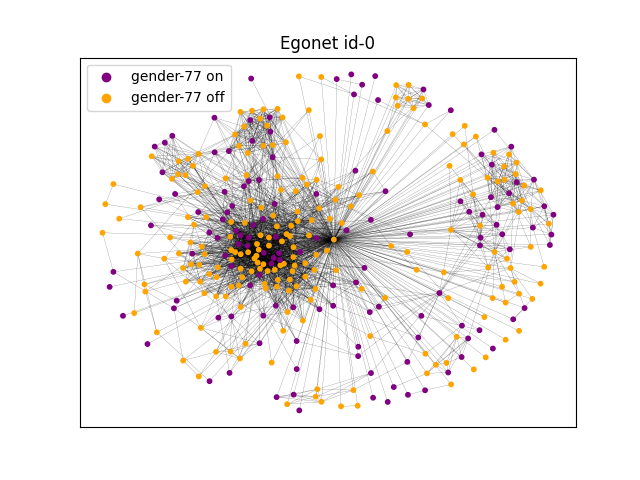
\includegraphics[width=\figwidth]{ego-0-by-gender.png}
	\caption{Egonet 0 with nodes coloured by gender}
	\label{fig:ego-0-by-gender}
\end{figure}

We use an SBM model with $k=2$ communities (1: gender-77 on and 2: gender-77 off) to model the egonet and perform a three-way hypothesis test on the parameters of the connectivity Matrix $W$.
%
\begin{equation}
	W = \begin{bmatrix}
		p_1 & q \\
		q & p_2
	\end{bmatrix}
\end{equation}

Therefore, $p_1$ is the probability that two vertices of gender-77 are connected, $q$ is the crossover probability and $p_2$ is the connection probability within the gender-78 community. The results of the hypothesis tests are given in table \ref{tab:egonet-0-hyp-tests} alongside p-values (we choose a 95\% significance level to reject the null). However, in some cases the test statistics were so extreme that the p-value saturated to 0.
%
\begin{table}[!h]
	\centering
	\begin{tabular}{c c c c c}
		$n_1$                & $n_2$                & $\hat{p_1}$ & $\hat{q}$ & $\hat{p_2}$       \\ \hline
		130 & 218 & $8.13 \times 10^{-2}$ & $7.66 \times 10^{-2}$ & $10.6 \times 10^{-2}$
	\end{tabular}
	\caption{Egonet-0 properties and parameter estimates}
	\label{tab:egonet-0-props}
\end{table}

\begin{table}[!h]
	\centering
	\begin{tabular}{cccccc}
		Test & $H_0$                & $H_1$                & p-value & $H_0$ rejected       \\ \hline
		1    & $p_1 = q$            & $p_1 \neq q$         & 0.158 &  No                \\
		2    & $p_1 = p_2$ & $p_1 \neq p_2$ & 0.000 & Yes \\
		3    & $q = p_2$ & $q \neq p_2$ &  0.000 & Yes
	\end{tabular}
	\caption{Egonet-0 hypothesis tests that gender influences friendship formation}
	\label{tab:egonet-0-hyp-tests}
\end{table}

Test 2 being rejected gives evidence that one gender has on average more friends from their own gender. We see that gender-78 people (community 2) have on average more friends ($\hat{p_2} > \hat{p_1}$ in table \ref{tab:egonet-0-props}). The rejection of the null in test 3 gives evidence that gender-78 treat gender-77 people differently to their own gender. Indeed, a gender-78 person is more likely to be friends with a fellow 78-er than with a 77-er. However, we do not reject the null in test 1 so there is insufficient evidence to claim the reverse (that 77-ers tend to stay away from 78-ers). Nevertheless, these are results on a single egonet so can hardly be generalised to society as a whole. However, the exercise has highlighted some interesting points:

\begin{enumerate}
	\item The hypothesis test framework does not quantify the magnitude of the difference just whether or not a difference exists.
	\item As the degree $n$ increases, the p-values will necessarily become more extreme.
	\item The method relies on the analyst to specify the features of interest so results may be misleading if third variables are missing from the analysis.
\end{enumerate} 

To address these shortcomings we instead approach the problem from a different angle. For now we have been given a graph with fully labelled vertices and ask if a given feature affect the structure. Instead, we could take a graph and partition into communities first (without using feature information) and then ask which features most reliably explain the partition. For that we need a way of detecting structure.

\section{Detecting Structure}

This is the problem of recovering the communities from the graph $\Gcal$. We use the notation $\hat{X}$ to denote the produced estimate of the community labels for the $n$ vertices. Obviously, if the SBM is symmetric then we must allow for an arbitrary relabelling of the communities $r: \{1, 2 \dots k\} \mapsto \{1, 2 \dots k\}$ before we compare the agreement of the two vectors $\hat{X}$ and $X$. The agreement $A$ and normalised agreement $\tilde{A}$ between two vectors $x, y$ are computed as below:
%
\begin{align}
	A(x, y) &= \max_r \frac{1}{n} \sum_{i=1}^{n} \one (x_i, r(y_i)) \\
	\tilde{A}(x, y) &= \max_r \frac{1}{k} \sum_{i=1}^{k} \frac{1}{n_i} \sum_{v \in \Omega_i(x)} \one(x_v, r(y_v))
\end{align}

The normalised agreement is important for asymmetric SBMs as it takes the agreement averaged over communities rather than vertices. We define 4 recovery regimes (plus the trivial no recovery), such that the following holds (adapted from Abbe \cite{Abbe}):

\begin{definition}
	For $(X, \Gcal) \sim \textrm{SBM}(m, p, W)$ the following recovery requirements are solved if there exists an algorithm which takes $\Gcal$ and input and outputs a vector of classifications $\hat{X} = \hat{X}(\Gcal)$ such that as $n \rightarrow \infty$:
	\begin{itemize}
		\item \textbf{Exact recovery:} $Pr\{A(X, \hat{X}) = 1\} = 1 - o(1)$ correct classification recovered almost surely
		\item \textbf{Almost exact recovery:} $Pr\{A(X, \hat{X}) = 1 - o(1)\} = 1 - o(1)$ vanishing fraction misclassified almost surely
		\item \textbf{Partial recovery:} $Pr\{\tilde{A}(X, \hat{X}) \geq \alpha\} = 1 - o(1), 1 > \alpha > 1/k$ better than choosing from uniform prior
		\item \textbf{Weak recovery:} $Pr\{\tilde{A}(X, \hat{X}) \geq 1/k + \epsilon \} = 1 - o(1), \epsilon > 0$ marginally better than choosing from uniform prior
		\item \textbf{No recovery:} graph provides no information as to class labels
	\end{itemize}
	Where $o(1)$ denotes a family of functions that tend to 0 as $n \rightarrow \infty$. The regime $\Gcal$ occupies depends on the parameters of the SBM. Each recovery regime is weaker than the one above it so Exact recovery implies weak recovery is possible..
\end{definition}

We choose to focus on weak recovery as it is the least strict of all regimes and in algorithms for weak recovery can solve stricter recovery regimes too. One of the most promising weak recovery algorithms is called Acyclic Belief Propagataion (ABP). We skim over the details here and merely represent our form of the algorithm, adapted from \cite{Linear-ABP}. ABP(r, T) on a graph $\Gcal$ with vertex set $\Vcal = \Vcal(\Gcal)$ and edge set $\Ecal = \Ecal(\Gcal)$:

\begin{enumerate}
	\item Initialise messages for $(v, v')$:
	\subitem $y^{(0)}_{v' \rightarrow v} \leftarrow \Gaussian(0, 1)$
	\item Iterate for $1 \leq t \leq T$ and for $(v, v') \in \Ecal$:
	\subitem compute average $s^{(t-1)} \leftarrow \frac{1}{2|E|} \sum_{(v, v') \in \Ecal} y^{(t-1)}_{v' \rightarrow v}$
	\subitem recentre messages $z^{(t-1)}_{v' \rightarrow v} \leftarrow y^{(t-1)}_{v' \rightarrow v} - s^{(t-1)}$ 
	\subitem sum incoming $y^{(t)}_{v' \rightarrow v} \leftarrow \sum_{(v', v'') \in \Ecal \setminus \{v\}}z^{(t-1)}_{v'' \rightarrow v'}$
	\subitem if $(v''' \rightarrow v \rightarrow v')$ on cycle of length $r' \leq r$ then correct:
	\subsubitem $y^{(t)}_{v' \rightarrow v} \leftarrow y^{(t)}_{v' \rightarrow v} - \sum_{(v, v'') \in \Ecal \setminus \{v', v'''\}}z^{(t-r')}_{v'' \rightarrow v'}$
	\item Assignment, for all $v \in V$:
	\subitem Sum incoming $y_v^{(T)} = \sum_{(v, v') \in \Ecal} y^{(t)}_{v' \rightarrow v}$
	\subitem Assign labels $\sigma_v = 1$ if $y_v^{(T)} > 0$ and $0$ otherwise
\end{enumerate}

We implement this algorithm in Python and apply it to the Facebook Egonets described earlier. 

\section{Verifying Structure}
\subsection{Single Sample against known mean}
We start with the simple case of determining whether or not a coin is fair. Each coin flip can be represented by a random variable with a Bernoulli distribution $X_i \sim Bern(p)$. Each coin can result in either a Tails or a Heads denoted by $X_i \in \{0, 1\}$. We toss the coin $n$ times leading us to a set $\left\{ X_i \right\}_{i=1}^{n}$. We wish to test the null hypothesis $p=p_0$ against the alternative. We shall keep the $p_0$ notation for generality, though for a fair coin we require $p_0=1/2$.
%
\begin{align*}
H_0:& \quad p = p_0 \\
H_1:& \quad p \neq p_0
\end{align*}
%
We denote the number of heads with the random variable $K \coloneqq \sum_{i=1}^{n} X_i \sim Bern(p, n)$. For a particular experiment we observe $K=k$. We employ a standard likelihood ratio test. The test statistic $t_n$ is calculated as the log-likelihood ratio of observing $K=k$ under $H_1$ and $H_0$.
%
\begin{equation}
t_n \coloneqq \log \frac{\lik(H_1)}{\lik(H_0)}
= \log \frac{\max_p P(K=k|p)}{P(K=k|p=p_0)}
\end{equation} 
%
We note that since $K$ is distributed as a binomial, $P(K=k|p)=\binom{n}{k}p^k(1-p)^{n-k}$. If we can vary $p$, this probability is maximised for $p=\hat{p} \coloneqq k/n$. Therefore, the test statistic is given by.
%
\begin{equation}
t_n = \log \frac{\binom{n}{k} \hat{p}^k (1 - \hat{p})^{n-k}}{\binom{n}{k} p_0^k (1 - p_0)^{n-k}}
=  \log \frac{ \hat{p}^k (1 - \hat{p})^{n-k}}{ p_0^k (1 - p_0)^{n-k}}
\end{equation}
%
The combinatoric term $\binom{n}{k}$ cancels out. This implies that the order in which the heads land does not matter when determining the fairness of the coin. We can work the above expression into a more usable form:
%
\begin{align}
t_n =& k \log \frac{\hat{p}}{p_0} + (n-k) \log \frac{1 - \hat{p}}{1 - p_0} \nonumber \\
=& n \left( \hat{p} \log \frac{\hat{p}}{p_0} + (1-\hat{p}) \log \frac{1 - \hat{p}}{1-p_0} \right) \nonumber \\
=& n \kl \left(Bern(\hat{p}) || Bern(p_0) \right)
\end{align}
%
Where $\kl(f | g) \coloneqq \sum_{x \in \Xcal} f(x) \log \frac{f(x)}{g(x)}$ is the Kullback-Leibler divergence between two arbitrary probability mass functions $f$ and $g$. This is also called the relative entropy. The KL divergence has the property that:
%
\begin{equation}
\kl (f || g) \geq 0 \quad \text{with equality iff} \quad f(x) = g(x) \quad \forall x \in \Xcal
\end{equation}
%
We can exploit this result for the case that $f \approx g$ to obtain a simplified expression for the KL divergence. We begin by defining $\delta (x) \coloneqq f(x) - g(x)$. We are interested in the region where $\delta$ is small. We start by substituting for $f=\delta + g$ and then taking the Taylor expansion of $\log 1+x$.
%
\begin{align*}
\kl(f||g) &= \sum_{x \in \Xcal} (\delta + g) \log \left(1 + \frac{\delta}{g} \right) \\
&= \sum_{x \in \Xcal} (\delta + g) \left( \frac{\delta}{g} - \frac{\delta^2}{2g^2} + O(\delta^3) \right) \\
&= \sum_{x \in \Xcal} \delta + \frac{1}{2} \sum_{x \in \Xcal} \frac{\delta^2}{g} + O(\delta^3) \\
&= \frac{1}{2} \sum_{x \in \Xcal} \frac{\delta^2}{g} + O(\delta^3) \\
&= \frac{1}{2} \chi^2(f||g) + O(\delta^3)
\end{align*}
%
Where the summation over $\delta$ evaluates to 0 because $\delta$ is the difference of two valid p.m.f's which each sum to 1 over $x \in \Xcal$. We are able to neglect the $O(\delta^3)$ terms for $f$ very close to $g$ we shall see what this means later. $\chi^2(f||g)$ is known as the chi-squared distance between two distributions and is defined simply as $\chi^2(f||g) \coloneqq \sum_{x \in \Xcal} (f-g)^2/g$. We now investigate the chi-squared divergence for $f = Bern(p)$ and $g = Bern(q)$.
%
\begin{align*}
\chi^2(Bern(p)||Bern(q)) &= \frac{(p-q)^2}{q} + \frac{((1-p)-(1-q))^2}{1-q} \\
&= \frac{(p-q)^2}{q(1-q)} \\
&= \left(\frac{p-q}{\sqrt{q(1-q)}}\right)^2
\end{align*}
%
Now we can exploit these results to get a workable expression for the test statistic $t_n$.
%
\begin{align*}
t_n &= n \kl \left(Bern(\hat{p}) || Bern(p_0)\right) \\
	&= \frac{n}{2} \chi^2 \left(Bern(\hat{p}) || Bern(p_0) \right) + nO(\delta^3) \\
	&= \frac{1}{2} \left( \frac{\hat{p} - p_0}{\sqrt{p_0(1-p_0)/n}} \right)^2 + \epsilon
\end{align*}
%
So far we have been treating $t_n$ as deterministic but it is merely an observation a random variable. To make this distinction clear we shall use upper-case to refer to random variables. Therefore, we have that the random variable $T_n$ is a function of $\hat{P} \coloneqq K/n$. For large n, we can find the distribution of $\hat{P}$ by the Central Limit Theorem.
%
\begin{align*}
\hat{P} &= \frac{K}{n} = \frac{1}{n} \sum_{i=1}^{n} X_i \\
H_0: \E[X_i] &= p_0, Var(X_i) = p_0(1-p_0) \\
\text{CLT, as }n \rightarrow \infty: \hat{P} &\sim \Gaussian\left(\mu=p_0, \sigma^2=p_0(1-p_0)/n\right) \\
\therefore \frac{\hat{P}-p_0}{\sqrt{p_0(1-p_0)/n}} = Z &\sim \Gaussian(\mu=0,\sigma^2=1)
\end{align*}
%
Therefore neglecting the error term $\epsilon$\footnote{See the Appendix for proof of negligibility}, we have that under $H_0$, for sufficiently large $n$.
%
\begin{align}
T_n = \frac{1}{2} Z^2 \sim \frac{1}{2} \chi_1^2
\end{align}
%
By the definition of the chi-squared distribution with one degree of freedom. To reject the null hypothesis $H_0$ at the $100(1-\alpha)\%$ confidence level, we require that $P(T_n \geq t_n | H_0) < \alpha$. In other words, a low probability of observing this result under the null hypothesis.

\subsection{Two samples equality of means}

We now complicate things by introducing a second coin, with throws denoted by $\{Y_i\}_{i=1}^{m}$ where we assume each throw is i.i.d Bernoulli with parameter $q$ ($Y_i \sim Bern(q)$). Note that the population sizes $n$ and $m$ may be different. We define $L \coloneqq \sum_{i=1}^{m} Y_i$ which is the analogue of $K$. We now set up our hypotheses to be:
%
\begin{align*}
H_0:& \quad p = q \\
H_1:& \quad p \neq q
\end{align*}
%
Proceeding as before we can derive a formula for the test statistic. This time we denote the test statistic by $t_N$ where $N \coloneqq n + m$.
%
\begin{align*}
t_N &\coloneqq \log \frac{\lik(H_1)}{\lik(H_0)}
= \log \frac{\max_{p,q} P(K=k|p) P(L=l|q)}{\max_p P(K=k|p) P(L=l|q=p)} \\
&= \log \frac
{\binom{n}{k} \hat{p}^k (1 - \hat{p})^{n-k} \binom{m}{l} \hat{q}^k (1 - \hat{q})^{m-l}}
{\binom{n}{k} \hat{r}^k (1 - \hat{r})^{n-k} \binom{m}{l} \hat{r}^l (1 - \hat{r})^{m-l}} \\
&= \log \frac
{ \hat{p}^k (1 - \hat{p})^{n-k}}
{ \hat{r}^k (1 - \hat{r})^{n-k}}
+ \log \frac{\hat{q}^k (1 - \hat{q})^{m-l}}{ \hat{r}^l (1 - \hat{r})^{m-l}}
\end{align*} 
%
Where, $\hat{p} \coloneqq k/n, \hat{q} \coloneqq l/m, \hat{r} \coloneqq (k+l)/(n+m) = (n\hat{p} + m\hat{q})/(n+m)$. Using the same tricks as before, we can express this in terms of the chi-squared distance between the various parameters:
%
\begin{align*}
t_N &= n \kl\left(Bern(\hat{p}) || Bern(\hat{r})\right)
+ m \kl\left(Bern(\hat{q}) || Bern(\hat{r})\right) \\ 
&\approx \frac{n}{2} \chi^2\left(Bern(\hat{p})||Bern(\hat{r}))\right)
+ \frac{m}{2} \chi^2\left(Bern(\hat{q})||Bern(\hat{r}))\right) \\
&= \frac{1}{2\hat{r}(1-\hat{r})} \left(
n(\hat{p} - \hat{r})^2 + m(\hat{q} - \hat{r})^2
\right) \\
&= \frac{1}{2\hat{r}(1-\hat{r})} \left(
n\left( \frac{m(\hat{p} - \hat{q})}{n+m}\right)^2 + 
m\left( \frac{n(\hat{q} - \hat{p})}{n+m}\right)^2
\right) \\
&= \frac{nm(\hat{p} - \hat{q})^2}{2\hat{r}(1-\hat{r})(n+m)} \\
&= \frac{1}{2} \left( \frac{\left(\hat{p} - \hat{q}\right)}{\sqrt{\hat{r}(1-\hat{r})(1/n+1/m)}}  \right)^2
\end{align*}
%
Under the null hypothesis $H_0$, we require $p=q(=\mu)$; we introduce this third variable $\mu$ to refer to the true mean to avoid ambiguity. Applying the central limit theorem (for sufficiently large $n$ and $m$) and combining Gaussians in the standard way, we have that:
%
\begin{equation*}
\begin{gathered}
\hat{P} \sim \Gaussian \left( \mu, \frac{\mu(1-\mu)}{n} \right) \\
\hat{Q} \sim \Gaussian \left(\mu, \frac{\mu(1-\mu)}{m} \right) \\
\hat{R} \sim \Gaussian \left(\mu, \frac{\mu(1-\mu)}{n+m} \right) \\
\therefore  \sqrt{\frac{nm}{\mu(1-\mu)(n+m)}} (\hat{P} - \hat{Q}) = Z \sim \Gaussian \left(0, 1 \right) \\
\delta \hat{R} \coloneqq \hat{R} - \mu \sim \Gaussian \left( 0, \frac{\mu(1-\mu)}{n+m} \right)
\end{gathered}
\end{equation*}
%
We almost have $T_n$ we just need to demonstrate that $\hat{R}(1-\hat{R})$ is sufficiently close to $\mu(1-\mu)$ for our purposes.
%
\begin{align*}
\hat{R}(1-\hat{R}) &= (\mu + \delta\hat{R})(1-(\mu + \delta \hat{R})) \\
&= \mu(1-\mu) + O(\delta\hat{R}) \\
\therefore \frac{1}{\hat{R}(1-\hat{R})} &= \frac{1}{\mu(1-\mu)} \left(\frac{1}{1+O(\delta\hat{R})}\right) \\
&= \frac{1}{\mu(1-\mu)} (1 + O(\delta\hat{R})) \\
&\approx \frac{1}{\mu(1-\mu)}
\end{align*}
%
We can neglect the terms of order $\delta\hat{R}$ and higher powers, as it is zero mean and for sufficiently large $n+m$ the variance approaches 0. Therefore, we have the desired expression for $T_N$.
%
\begin{equation}
T_N \approx \frac{1}{2} \left(
\sqrt{\frac{nm}{\mu(1-\mu)(n+m)}}
(\hat{P} - \hat{Q})
\right)^2 = \frac{1}{2} Z^2 \sim \frac{1}{2} \chi^2_1
\end{equation}
%
For this test we can also use the z-statistic instead of the t-statistic. Since the former is distributed like a Gaussian it may be easier to deal with.
\begin{align}
z_N = \frac{\hat{p} - \hat{q}}{\sqrt{\hat{r}(1-\hat{r})\left(1/n + 1/m\right)}} \sim \Gaussian(0, 1)
\end{align}


\section{Detecting Structure}
\subsection{ABP}

ABP(r, T) on a graph $G$ with vertex set $V = V(G)$ and edge set $E = E(G)$
\begin{enumerate}
	\item Initialise messages for $(v, v')$:
		\subitem $y^{(0)}_{v' \rightarrow v} \leftarrow \Gaussian(0, 1)$
	\item Iterate for $1 \leq t \leq T$ and for $(v, v') \in E$:
		\subitem compute average $s^{(t-1)} \leftarrow \frac{1}{2|E|} \sum_{(v, v') \in E} y^{(t-1)}_{v' \rightarrow v}$
		\subitem recentre messages $z^{(t-1)}_{v' \rightarrow v} \leftarrow y^{(t-1)}_{v' \rightarrow v} - s^{(t-1)}$ 
		\subitem sum incoming $y^{(t)}_{v' \rightarrow v} \leftarrow \sum_{(v', v'') \in E \setminus \{v\}}z^{(t-1)}_{v'' \rightarrow v'}$
		\subitem if $(v''' \rightarrow v \rightarrow v')$ on cycle of length $r' \leq r$ then correct:
			\subsubitem $y^{(t)}_{v' \rightarrow v} \leftarrow y^{(t)}_{v' \rightarrow v} - \sum_{(v, v'') \in E \setminus \{v', v'''\}}z^{(t-r')}_{v'' \rightarrow v'}$
	\item Assignment, for all $v \in V$:
		\subitem Sum incoming $y_v^{(T)} = \sum_{(v, v') \in E} y^{(t)}_{v' \rightarrow v}$
		\subitem Assign labels $\sigma_v = 1$ if $y_v^{(T)} > 0$ and $0$ otherwise
\end{enumerate}

\section{Composite Approaches}

\section{Appendix}

\subsection{Proving H.O.T can be neglected}
We have shown that under the null hypothesis, that for sufficiently large $n$, $(\hat{P}-p_0) \sim \Gaussian(0, \beta/n)$ for some positive finite constant $\beta$ (in this case $\beta = p_0(1-p_0)$ but we just require finiteness for this proof). Therefore, $Q \coloneqq \sqrt{n} (\hat{P} - p_0) \sim \Gaussian(0,\beta)$. Manipulating our expression for the error term $\epsilon$ we can show that it can be expressed as a sum of 
%
\begin{equation}
\begin{gathered}
\epsilon = n O(\delta^3) \\
\therefore |\epsilon| \leq n \sum_{i=0}^{\infty} \alpha_i|\hat{P} - p_0|^{3+i} 
\quad \text{for some finite constants } \alpha_i \geq 0 \\
|\epsilon| \leq \sum_{i=0}^{\infty} \alpha_i n^{-\frac{1+i}{2}}( \sqrt{n}|\hat{P} - p_0|)^{3+i} \\
|\epsilon| \leq \sum_{i=0}^{\infty} \alpha_i n^{-\frac{1+i}{2}}|Q|^{3+i}
\end{gathered}
\end{equation}
%
We know that $Q$ is a Gaussian of zero mean and finite variance, therefore $|Q|$ will be a finite value. However, we see that it is scaled by a negative power of $n$, therefore for sufficiently large $n$ we have that the error term asymptotes to 0. To be precise:
%
\begin{equation}
\begin{gathered}
\lim_{n \rightarrow \infty} P(|\epsilon| < \eta) = 1 \text{ for arbitrarily small } \eta \ge 0
\end{gathered}
\end{equation}

\nocite{*}
\printbibliography

\end{document}
